\section{Relational cross-attention and the abstractor module}\label{sec:abstractor_module}

At a high level, the primary function of an Abstractor is to compute abstract relational features of its inputs.\footnote{In this paper, we will use the name `Abstractor' to refer to both the module and to model architectures which contain the Abstractor module as a main component.} That is, given a sequence of input objects $x_1, \ldots, x_\m$, the Abstractor learns to model a relation $r(\cdot, \cdot)$ and computes a function on the set of pairwise relations between objects ${\{ r(x_i, x_j) \}}_{ij}$. At the heart of the Abstractor module is an inductive bias we call the \textit{relational bottleneck}, that disentangles relational information from the features of individual objects.

\subsection{Modeling relations as inner products}\label{ssec:relations_as_inner_prods}

A ``relation function'' maps a pair of objects $x_1, x_2 \in \calX$ to a vector representing the relation between the two objects. We model pairwise relations as inner products between appropriately encoded (or `filtered') object representations. In particular, we model the pairwise relation function $r(\cdot, \cdot) \in \mathbb{R}^{d_r}$ in terms of $d_r$ learnable `query' encoders $\phi_q^{1}, \ldots, \phi_{q}^{d_r}$ and `key' encoders $\phi_k^{1}, \ldots, \phi_{k}^{d_r}$,
\begin{equation}\label{eq:inner_prod_rel}
    r(x, y) = \left(\langle \phi_q^{1}(x), \phi_k^{1}(y) \rangle, \langle \phi_q^{2}(x), \phi_k^{2}(y) \rangle, \ldots, \langle \phi_q^{d_r}(x), \phi_k^{d_r}(y) \rangle \right) \in \mathbb{R}^{d_r}.
\end{equation}
% A common choice is to model $(\phi_q^i, \phi_k^i)_{i\in [d_r]}$ as linear or affine maps. Considering all pairwise relations yields a \textit{relation tensor}, $R = \left[r(x_i, x_j)\right]_{i,j} \in \mathbb{R}^{\m \times \m \times d_r}$.

% AWNI: removed this for space. can add this back (or some version of it) if we think it's important. focusing on santoro1 for an entire paragraph might be distracting; although it does help explain the relational bottleneck. also worth noting, the current relconvnet paper has a similar paragraph.

% In principle, relations could be modeled by an arbitrary learnable function applied to the concatenation of the features of a pair of objects.~\citep{santoro1} takes this approach and models relations through MLPs applied to the concatenation of the features of a pair of objects. This approach is versatile in principle and can work given enough data. However, modeling relations as inner products has some important advantages. First, it induces a pressure on the resultant representations to encode relational information and constricts the leakage of information about individual objects. When relations are modeled as $g_\theta(\mathrm{concat}(x_1, x_2))$, for some parameterized function class $g_\theta$, there is no pressure or restriction that this function represents relations between the two objects---it can just as well represent information about the objects' features individually.

Modeling relations as inner products $\iprod{\phi_q(x)}{\phi_k(y)}$ ensures that the result represents a comparison between the two objects' features. More precisely, inner product relations induce a geometry on the object space $\calX$, with notions of distance, angles, and orthogonality.~\citet{altabaaApproximationRelationFunctions2024} analyzes the approximation properties of inner products of neural networks for relation functions.
%Modeling relations as inner products is an approach that has been explored in previous work on relational architectures (e.g.,~\citep{esbn,kerg2022neural}) and has been shown to be a useful inductive bias on several discriminative relational tasks.

Considering all pairwise relations yields a \textit{relation tensor}, $R = \left[r(x_i, x_j)\right]_{i,j} \in \mathbb{R}^{\m \times \m \times d_r}$.

\subsection{Relational Cross-Attention}\label{ssec:relational_crossattention}

The core operation in a Transformer is attention. For an input sequence $X = (x_1, \ldots, x_\m) \in \reals^{\m \times d}$, self-attention transforms the sequence via, $ X' \gets \mathrm{Softmax}({\phi_q(X)} {\phi_k(X)}^\top) \, \phi_v(X)$, where $\phi_q, \phi_k, \phi_v$ are functions applied independently to each object in the sequence.
% (i.e., $\phi(X) = (\phi(x_1), \ldots, \phi(x_\m))$).
% Typically, those are linear or affine functions.
% , with $\phi_q, \phi_k$ having the same dimensionality so we can take their inner product.
Note that $R := {\phi_q(X)} {\phi_k(X)}^\top$ is a relation matrix in the sense defined above. Self-attention admits an interpretation as a form of ``neural message-passing''~\citep{gilmer2017neural} as follows
\begin{equation}\label{eq:self_attn_message_passing}
    x_i' \gets \mathrm{MessagePassing}\paren{\set{(\phi_v(x_j), R_{ij})}_{j \in [\m]}} = \sum_{j} \bar{R}_{ij} \phi_v(x_j),
\end{equation}
where $m_{j \to i} = (\phi_v(x_j), R_{ij})$ is the message from object $j$ to object $i$, encoding the sender's features $\phi_v(x_j)$ and the relation between the two objects $R_{ij} = \iprod{\phi_q(x_i)}{\phi_k(x_j)}$. Here, $\bar{R} = \mathrm{Softmax}\paren{R}$ is the softmax-normalized relation matrix. Hence, the processed representation obtained by self-attention is an entangled mixture of relational information and object-level features.
% Thus, self-attention is a form of message-passing where the message from object $j$ to object $i$ is an encoding of object $j$'s features weighted by the (softmax-normalized) relation between the two objects. As a result, the processed representation obtained by self-attention involves some relational information. However, this relational information is entangled with object-level features.

Our goal is to learn relational representations which are abstracted away from object-level features in order to achieve more sample-efficient learning and improved generalization in relational reasoning. This is not naturally supported by the entangled representations produced by standard self-attention. We achieve this via a simple modification of attention---we replace the values $\phi_v(x_i)$ with vectors that \textit{identify} objects, but do not encode their features. We call those vectors \textit{symbols}. Hence, the message sent from object $j$ to object $i$ is now $m_{j \to i} = (s_j, R_{ij})$, the relation between the two objects, together with the symbol identifying the sender object,
\begin{equation}\label{eq:relational_crossattn_message_passing}
    A_i \gets \mathrm{MessagePassing}\paren{\set{(s_j, R_{ij})}_{j \in [\m]}} = \sum_{j} \bar{R}_{ij} s_j.
\end{equation}
Symbols act as abstract references to objects, akin to pointers in traditional symbolic architectures. They do not encode information about the contents or features of the objects, but rather \textit{refer} to objects.
This results in improved sample efficiency and generalization by restricting the search space of computations, and allowing abstraction through shared symbols.
We call the vectors $\{s_i\}$ `symbols' in the same sense that we call `$x$' a symbol in an equation like $y = x^2$---they reference an object with an unspecified value.
%  via their position. The symbols $S = (s_1, s_2, \ldots)$ can be either learned parameters of the model or nonparametric positional embeddings.
Suppose for now that each object $x_i$ is assigned a symbol $s_i$ in a manner that satisfies this property. We will discuss symbol-assignment mechanisms in the next subsection.
% The difference is that the symbols here are `distributed representations' (i.e., vectors), leading to a novel perspective on the long-standing problem of neural versus symbolic computation.

This modification yields a variant of attention that we call \textit{relational cross-attention} (RCA), given by
\begin{equation}\label{eq:relational_crossattn}
    A \gets  \sigma_{\mathrm{rel}}\paren{\phi_q(X) \, {\phi_k(X)}^\top} S,
\end{equation}
where $S = (s_1, \ldots, s_\m)$ are the symbols, $\sigma_{\mathrm{rel}}$ is the relation activation function, and $\phi_q, \phi_k$ correspond to the query and key transformations. When the relation activation function $\sigma_{\mathrm{rel}}$ is softmax, this corresponds to $\mathrm{Attention}(Q \gets X,\, K \gets X,\, V \gets S)$. In contrast, self-attention corresponds to $\mathrm{Attention}(Q \gets X,\, K \gets X,\, V \gets X)$, mixing relational information with object-level features.

We observe in our experiments that allowing $\sigma_{\mathrm{rel}}$ to be a configurable hyperparameter can lead to performance benefits in some tasks. Softmax has the effect of normalizing the relation between a pair of objects $(i,j)$ based on the strength of $i$'s relations with the other objects in the sequence. In some tasks this is useful. In other tasks, this may mask relevant information, and element-wise activations (e.g., tanh, sigmoid, or linear) may be more appropriate.

Relational cross-attention implements a type of information bottleneck, that we call the ``relational bottleneck'', wherein the resultant representation encodes only relational information about the object sequence (\Cref{fig:attn_mechanisms}) and does not encode information about the features of individual objects.
% \footnote{The diagonal entries of the relation matrix $R_{ii} = \iprod{\phi_q(x_i)}{\phi_k(x_i)}$ encode information about individual objects. This can be interpreted as a leakage of non-relational information. It's possible to implement a stricter relational bottleneck by masking the diagonal entries of $R$, but we find this to be unnecessary in our experiments.}. 
This enables a branch of the model to focus purely on modeling the relations between objects, yielding greater sample-efficiency in tasks that rely on relational reasoning.

% \begin{remark}
%     We call this operation ``relational cross-attention'' because 1) it computes relational representations, and 2) when attending to the input objects,  only
%     relational information, not sensory information, is allowed to cross over, since 
%     the values are input-independent. \awni{I was thinking (1) explains `relational' and (2) explains `cross-attention'. But we might want to remove this since we're tight on space and it's not really necessary.}
% \end{remark}

Multi-dimensional relations can be modeled through multi-head relational cross-attention. In our experiments, $\phi_q^i, \phi_k^i$ are linear maps $W_q^{i}, W_k^{i}$, and multi-head relational cross-attention is given by
\begin{equation}
    \begin{split}
        % \mathrm{RelationalCrossAttention}(X, S) &= \mathrm{MultiHeadAttention}\paren{Q \gets X,\, K \gets X,\, V \gets S} \\
        \mathrm{RelationalCrossAttention}(X, S) &= \mathrm{concat}\paren{A^{1}, \ldots, A^{d_r}} W_o, \\
        \text{where } A^i &= \sigma_{\mathrm{rel}}\paren{(X \, W_q^{i}) {(X \, W_k^{i})}^\top} S \, W_o^{i} .
    \end{split}
\end{equation}

\begin{figure}
    \begin{subfigure}[b]{0.5\textwidth}
        \centering
        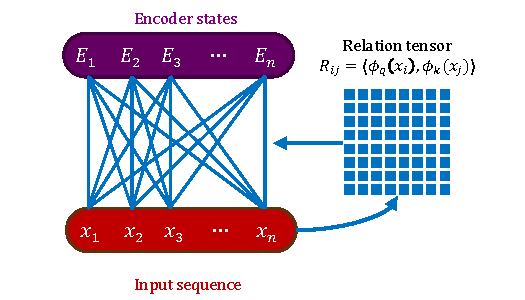
\includegraphics[width=\textwidth]{figures/self_attn_fig.pdf}
        \caption{$E \gets \mathrm{SelfAttention}(X)$}\label{fig:self_attention}
    \end{subfigure}
    \hfill
    \begin{subfigure}[b]{0.5\textwidth}
        \centering
        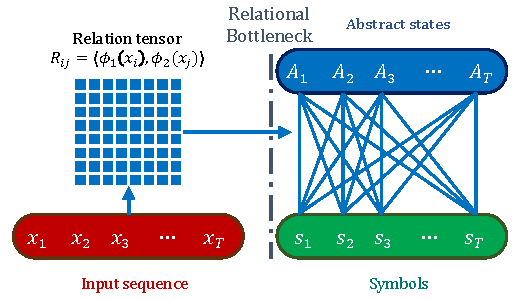
\includegraphics[width=\textwidth]{figures/rel_crossattn_fig.pdf}
        \caption{$A \gets \mathrm{RelationalCrossAttention(X, S)}$}\label{fig:relational_cross_attention}
    \end{subfigure}
    \caption{Comparison of relational cross-attention with self-attention. Red represents object-level features, blue represents relational features, and purple represents mixed representations. Relational cross-attention computes relational information disentangled from the features of individual objects.}\label{fig:attn_mechanisms}
    \vskip-15pt
\end{figure}

\subsection{Symbol assignment mechanisms}\label{ssec:symbol_assignment}
Abstraction relies on the assignment of symbols to individual objects without directly encoding their features. We propose three different mechanisms for assigning symbols to objects.

\textbf{Positional symbols.} The simplest symbol assignment mechanism is to assign symbols to objects sequentially based on the order they appear in the sequence. That is, we maintain a library of symbols $S_{\mathrm{lib}} = (s_1, \ldots, s_{\mathtt{max\_len}}) \in \reals^{\mathtt{max\_len} \times d_{\mathrm{model}}}$, and assign the symbol $s_i$ to the $i$-th object. The symbol library $S_\mathrm{lib}$ can be either learned parameters of the model or fixed positional embeddings. %While very simple, positional symbols often work well in practice.

\textbf{Position-relative symbols.} Similar to relative positional embeddings~\citep{shaw2018self,kazemnejadImpactPositionalEncoding2023}, we can compute relational cross-attention with position-relative symbols via $A_i \gets \sum_j R_{ij} s_{j-i}$, where the symbol library is $S_{\mathrm{lib}} = \paren{\ldots, s_{-1}, s_0, s_1, \ldots}$.

\textbf{Symbolic attention.} In this case we learn a library of symbols $S_{\mathrm{lib}} = (s_1, \ldots, s_{n_s}) \in \reals^{n_s \times d_{\mathrm{model}}}$ together with associated ``binding vectors'' $B_{\mathrm{lib}} = (b_1, \ldots, b_{n_s})$, where $n_s$ is the number of symbols in the library. Through an attention mechanism, symbols are bound to objects $x_i$ based on their relations to the symbol binding vectors. A multi-head variant of symbolic attention is naturally defined by concatenating the symbols retrieved for each head. Formally, 
\begin{equation}
    \begin{split}
        \mathrm{SymbolicAttention}(X) &= \mathrm{concat}\paren{S^{(1)}, \ldots, S^{(n_h)}}, \\
        S^{i} &= \mathrm{Softmax} \paren{(X W_q^{i}) {B_{\mathrm{lib}}^{i}}^\top} S_{\mathrm{lib}}^{i}.
    \end{split}
\end{equation}
In terms of representational capacity, this is similar to cross-attending to the symbol parameters $S_{\mathrm{lib}}$.
% (with the keys $W_k S_{\mathrm{lib}}$ taking the role of the binding vectors $B_{\mathrm{lib}}$)
Note that symbolic attention weakens the relational bottleneck since object-level features are used to retrieve a symbol for each object. However, 
the symbols are shared across objects and sequences, and the dependence is only with respect to a low-dimensional projection of the object-level features, which we may think of as encoding the object's ``syntactic role.'' Encoding such information in the symbols allows identifying objects by their role, rather than merely their position or relative position.

The choice of symbol assignment mechanism determines the way in which relational information is encoded in the abstract states. For example, with positional symbols, $A_i$ encodes the relations between object $i$ and each object $j$, identifying $j$ by its position (or relative position in the case of position-relative symbols). In contrast, with symbolic attention, each object $j$ is identified by its ``syntactic role,'' as determined by its relation to the binding vectors.

%TODO: add more in-depth discussion to appendix. including role of self-attention prior, in certain architectures, the strength of the relational bottleneck etc. Examples of what we think of "roles" in symbolic attention being. also discuss intuition.
\subsection{The Abstractor module}\label{ssec:abstractor_module}

We now describe the Abstractor module. Like the Encoder in a Transformer, this is a module that processes an input sequence of objects $X = \paren{x_1, \ldots, x_\m}$ producing a processed sequence of objects $A = \paren{A_1, \ldots, A_\m}$ that represents features of the input sequence. In an Encoder, the output objects represent a mix of object-level features and relational information. In an Abstractor, the output objects are abstract states that represent relational information, abstracted away from the features of individual objects. The core operation in an Abstractor module is relational cross-attention. Mirroring an Encoder, an Abstractor module can comprise several layers, each composed of relational cross-attention followed by a feedforward network. Optionally, residual connections and layer-normalization can be applied as suggested by~\citet{vaswani2017attention}\footnote{Layer-normalization can also be applied \textit{before} relational cross-attention, as in the pre-LN Transformer~\citep{xiong2020layer}.}. The algorithmic description is presented in~\Cref{alg:abstractor_module}. In~\Cref{sec:abstractor_approx_theory}, we theoretically study the approximation properties of the Abstractor module, showing that it is a universal approximator of relation functions.

\begin{algorithm}[ht!]
	\caption{Abstractor module}\label{alg:abstractor_module}
	\SetKwInOut{Input}{Input}
	% \SetKwInOut{Output}{Output}
	% \SetKwInOut{LearnableParams}{Learnable parameters}
	% \SetKwInOut{HyperParams}{Hyperparameters}

	\Input{object sequence: $\bm{X} = (x_1, \ldots, x_\m) \in \reals^{\m \times d}$ }
	\vspace{1em}

    $A^{(0)} \gets \mathrm{SymbolicAttention(X)}$ \quad \texttt{// or, $A^{(0)} \gets S_{1:\m}$, for positional symbols}

	\For{\(l \gets 1\) \KwTo \(L\)}{

        $A^{(l)} \gets \mathrm{RelationalCrossAttention}\paren{X, A^{(l-1)}}$

        $A^{(l)} \gets A^{(l)} + A^{(l-1)}$ \quad \texttt{// residual connection (optional)}

        $A^{(l)} \gets \mathrm{LayerNorm}(A^{(l)})$ \quad \texttt{// (optional; can also be done pre-RCA)}

        $A^{(l)} \gets \mathrm{FeedForward}\paren{A^{(l)}}$

        % \vspace{1em}
        % \texttt{optionally, self-attention:}

        % $A^{(l)} \gets \mathrm{SelfAttention}\paren{A^{(l)}}$

        % $A^{(l)} \gets A^{(l)} + A^{(l-1)}$ \quad \texttt{residual connection (optional)}

        % $A^{(l)} \gets \mathrm{LayerNorm}(A^{(l)})$ \quad \texttt{(optional)}

        % $A^{(l)} \gets \mathrm{FeedForward}\paren{A^{(l)}}$
    }

    \textbf{Output:} $A^{(L)}$

\end{algorithm}

The hyperparameters of an Abstractor module include the number of layers $L$, the relation dimension $d_r$ (i.e., number of heads),  the projection dimension $d_k$ (i.e., key dimension), the relation activation function $\sigma_{\mathrm{rel}}$, and the model dimension $d_{\mathrm{model}}$. The learnable parameters, at each layer, are the projection matrices $W_q^{i}, W_k^{i} \in \reals^{d_{\mathrm{model}} \times d_k}, \ i \in [d_r]$, the symbol library $S_{\mathrm{lib}}$, and the parameters of the feedforward network. In our experiments, we use a 2-layer feedforward network with a hidden dimension $d_{\mathrm{ff}}$ and ReLU activation. The implementation in the publicly available code adds a few additional hyperparameters, including whether to restrict the learned relations to be symmetric (via $W_q^{i} = W_k^{i}$), and whether to apply self-attention after relational cross-attention (which enables exchange of relational information between abstract states).

% Observe that in the first layer of the Abstractor, the values in relational cross-attention are the input-independent symbols. In the following layers, the values are the abstract states from the previous layer. %In the next subsection we characterize the function class of 1-layer Abstractor modules. Computations in deeper Abstractor modules are more difficult to interpret in terms of the original input sequence, but, empirically, we find that deeper Abstractor modules can yield improvements in performance.